\scanpage{158}
% archive sheet number: 157
\diagram{\begin{tikzcd}[ampersand replacement=\&]
\pi_1(S,\xi)=\varprojlim\pi_1(S_i,\xi_i) \arrow[d] \\
G
\end{tikzcd}}
\[\pi_1(S,\xi)\qquad\bullet\]
\figure{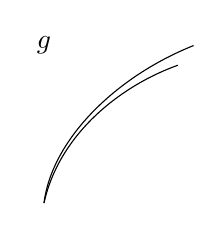
\begin{tikzpicture}
\node at (0,2) {$\mathfrak g$};
\draw (0,0) .. controls (.1,.8) and (.9,1.6) .. (1.9,2);
\draw (0,0) .. controls (.2,.9) and (1,1.5) .. (1.7,1.75);
\end{tikzpicture}}
\diagram{\begin{tikzcd}[ampersand replacement=\&,column sep=large]
\& \overline{k}_0 \arrow[d,no head] \\
\overline{k}_1 \arrow[r,no head] \arrow[d,no head] \& (\overline{k}_1,k_2) \arrow[d,no head] \\
\unsure{K_1|k_1} \arrow[r,no head,"{\text{``\unsure{infini|infinie}''}}"'] \arrow[d,no head] \& k_2 \\
k_1
\end{tikzcd}}
\figure{\begin{tikzpicture}\draw (0,.8)--(.05,.6);\draw (0,.2).. controls (.1,0) .. (.2,-.1);\draw (.5,.8)--(.65,.8);\end{tikzpicture}}
\diagram{\begin{tikzcd}[ampersand replacement=\&]
\& A' \& S \\
\bullet\ A \arrow[ur,no head] \arrow[r] \& A_i
\end{tikzcd}}
\figure{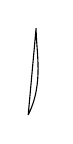
\begin{tikzpicture}\draw (0,0).. controls (.2,.4) and (.1,.8)..(.1,1.1)--(0,0);\end{tikzpicture}}
\[
\begin{aligned}
&\exists\ g\in G\\
&U\ \text{voisinage de }e\\
&(gu)^n\in H\ \text{pour tt }u
\end{aligned}
\]
\diagram{\begin{tikzcd}[ampersand replacement=\&]
A \arrow[r] \& B \\
S \& T \arrow[l] \\
S_i \& T_i \arrow[l] \\
\pi_1(S_i) \& \pi_1(T) \arrow[l]
\end{tikzcd}}
\[\mathfrak g_1\subset\mathfrak g_2\]
\[
\begin{gathered}
\deleted{H_1\unsure{\subset|\longleftarrow}\unsure{\widehat\Pi_c|\widehat H_2}}\\
H_1\unsure{,\subset|\subset}H_2\\
\cap\\G
\end{gathered}
\]
\diagram{\begin{tikzcd}[ampersand replacement=\&]G\arrow[r,leftrightarrow]\&G'\end{tikzcd}}
\figure{
\begin{tikzpicture}\draw[line width=2pt](0,0)--(.8,.5);\end{tikzpicture}}
\diagram{\begin{tikzcd}[ampersand replacement=\&]S\&S'\arrow[l]\end{tikzcd}}
\diagram{\begin{tikzcd}[ampersand replacement=\&]
\&\unsure{\Gamma|\mathscr T}\subset G\times G'\arrow[dl]\arrow[dr]\\
G\&\&G'
\end{tikzcd}}
\diagram{\begin{tikzcd}[ampersand replacement=\&]G\arrow[r]\&G'\end{tikzcd}}
\diagram{\begin{tikzcd}[ampersand replacement=\&,row sep=large]
\begin{gathered}\text{$\unsure{k|\ell}$-groupe de type \unsure{galoisien}}\\\text{avec groupes finis}\end{gathered}\arrow[d,"{\deleted{\unsure{\mathfrak g|F}}}"']\\
\begin{gathered}\text{systèmes projectifs \unsure{stricts}}\\\text{d'algèbres de Lie de}\\\text{dim finie sur }\mathbb Q_\ell\end{gathered}
\end{tikzcd}}
\figure{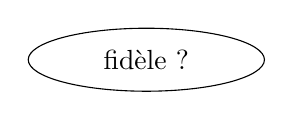
\begin{tikzpicture}\draw (0,0) ellipse (1.5 and .4);\node at (0,0){\unsure{fidèle} \unsure{?}};\end{tikzpicture}}
\uline{Lemme} le th est vrai pour
\[H_1\simeq\mathbb Z_\ell\]
\diagram{\begin{tikzcd}[ampersand replacement=\&,column sep=small,row sep=large]
\begin{gathered}\text{que }H_1\unsure{\subset_{\mathfrak g}|\subset_G|\subset}H_2\\
\text{i.e. }H_1\cap H_2\text{ est}\\\text{ouvert dans }H_1,\\\text{i.e. d'indice fini}\end{gathered}\arrow[r,Rightarrow]
\&\mathfrak g_1\subset\mathfrak g_2\arrow[r,"?"]
\&\begin{gathered}\text{tt \unsure{Germe|groupe}}\\\text{de ss-groupe}\\\text{à un paramètre de}\\H_1\\
\deleted{\text{qui a }\unsure{\text{sa}}\ \unsure{H_1}}\ \inserted{\text{est}}\ \unsure{\text{dans|en}}\ H_2\end{gathered}\arrow[d,Rightarrow,"{\deleted{\unsure{H_1}}\ \unsure{\text{cpt}}}"]\\
\&\begin{gathered}\text{par Lemme : si }H\subset G,\text{ et tt élém de }G\text{ a une puiss. en }H,\\\text{alors }H\text{ d'indice fini dans }G.\end{gathered}\arrow[ul,bend left=10,Rightarrow]
\&\begin{gathered}\text{tout}\ \text{élément de }H_1\\\text{a une puissance}\\\text{dans }H_2\end{gathered}
\end{tikzcd}}
\figure{\begin{tikzpicture}\draw (0,0)--(.5,.4);\draw(1.5,1)..controls(2,1.1)and(2,.7)..(2,.3);\draw (3,1) .. controls (4,1) and (3.3,.2)..(5,.2) -- (6.4,.2);\end{tikzpicture}}
